\documentclass[11pt]{article}

\usepackage[margin=1in]{geometry}
\usepackage{amsmath,amssymb}
\usepackage{graphicx}
\usepackage{booktabs}
\usepackage{natbib}
\usepackage{textcomp}
\usepackage{hyperref}
\hypersetup{colorlinks=true, linkcolor=blue, urlcolor=blue, citecolor=blue}

\title{Grid-Point Skill Is Not Eddy Skill: A Training-Objective Fix for the Double-Penalty Problem, With an Unexplained Resolution Sensitivity --- A Case Study in the Agulhas Current}
\author{}
\date{}

\begin{document}
\maketitle

\begin{abstract}
In a case study of the Agulhas Current, we show that a training-objective fix --- not architecture --- closes the gap between grid-point forecast skill and eddy-detection skill in machine-learned ocean forecasting. A convolutional U-Net beats persistence by an order of magnitude on grid-point skill, yet leaves eddy-detection recall essentially unchanged (92.66\% persistence vs. 92.69\% CNN control, $n=2{,}336{,}570$ true eddies pooled across 5 seeds): architecture reliably fixes eddy position error but not whether an eddy is detected at all --- the double-penalty problem \citep[]{Ebert2008,Gilleland2009}, surviving an order-of-magnitude architecture change. An amplitude-adjusted MSE loss (AMSE), adapting a spectral fix from global weather forecasting, closes this gap: pooled recall rises to 93.60\% (a $\approx$12\% relative reduction in missed eddies) and mean position error falls $\approx$12\%, consistent across 5 seeds and directionally confirmed against an independent altimetry eddy atlas (AVISO). This is not free --- AMSE costs 4.8--7.4 points of grid-point skill and reverses 20-day rollout stability from positive to negative at this resolution --- and the case study is scoped to one reanalysis product (GLORYS12V1), one chronological split, and one field-standard tracker (py-eddy-tracker); the CNN itself was chosen as primary architecture after a controlled comparison confirmed a Deep Operator Network's whole-domain design is unsuited to this fixed-grid task.

Two results remain open. Whether AMSE's gain specifically favors the anticyclonic Agulhas rings motivating this study, rather than eddies incidental to it, has reversed direction twice and is unresolved at this paper's primary resolution --- a gap in the paper's own reason for existing, not a peripheral loose end. And this project has caught and corrected four significant errors during development, including a 232$\times$ eddy-count undercount; we disclose this as grounds for reader skepticism rather than confidence earned by disclosure, and independent, outside-the-project reproduction of our central tables has not yet happened.
\end{abstract}

\section{Introduction}

The global ocean is a multiscale fluid system in which the majority of kinetic energy resides not in the mean circulation but in the mesoscale field --- rotating, coherent eddies tens to hundreds of kilometers across \citep[]{FerrariWunsch2009}. These eddies dominate oceanic variability at daily-to-weekly timescales and are estimated to hold roughly 80\% of the ocean's total kinetic energy \citep[]{Garabato2022}. In the Southern Ocean, the mesoscale eddy field accounts for more than half of the kinetic energy of the circulation and is the dominant mechanism for cross-frontal heat transfer in the Antarctic Circumpolar Current (NOAA GFDL, n.d.; \citealp{Gray2024}). Eddies are also central to the ocean carbon cycle: they act as conduits for heat, salt, carbon, and nutrients, and are estimated to enhance the oceanic CO$_2$ sink by roughly 10--14\% in major sequestration regions such as the Kuroshio Extension and Gulf Stream, with global carbon uptake potentially underestimated by as much as 233 Tg C per year when eddy contributions are unresolved \citep[]{Li2025}. The Agulhas Current, flowing poleward along the southern African coast before looping back on itself at the Agulhas Retroflection, is one of the most energetic mesoscale regions in the world ocean; the retroflection periodically sheds large, warm, salty rings that drift for months and carry heat and salt thousands of kilometers into the South Atlantic, forming a principal pathway of inter-ocean exchange between the Indian and Atlantic basins \citep[]{Lutjeharms2007,Zhu2021}. Despite this significance, Agulhas eddies remain poorly represented in Earth System Models because they occur at scales that are computationally expensive to resolve globally \citep[]{Smith2023}. Data-driven forecasting is an emerging alternative \citep[]{Heimbach2024}, and a global Swin-Transformer forecaster trained on the same underlying GLORYS reanalysis, WenHai \citep[]{Cui2025}, already reports that persistence is a strikingly strong baseline in this setting --- a state-of-the-art numerical model, GLO12v4, ``does not beat the persistent forecast except for the SST.''

A methodological gap sits underneath all of this work. Machine-learned ocean and weather forecasters are trained and evaluated almost exclusively against pointwise metrics --- RMSE, skill scores, anomaly correlation --- but a large spatial-forecast-verification literature has established that pointwise metrics systematically misjudge coherent, displaced features: a correctly shaped, correctly timed feature that is spatially offset from its true position is penalized twice, once as a missed observation and once as a false prediction, a phenomenon named the \textit{double-penalty problem} \citep[]{Ebert2008,Gilleland2009}. The remedy proposed in that literature is a neighborhood- or fractions-based verification metric that tolerates small displacements \citep[]{RobertsLean2008}; WenHai and the Gulf-Stream/Loop-Current forecaster OceanNet \citep[]{Chattopadhyay2024} both already address this problem \textit{at evaluation time}, using neighborhood-based or modified-Hausdorff-distance metrics rather than relying on RMSE alone. This paper's central methodological contribution is to instead fix the problem \textit{at training time} --- a direction \citet{Lagerquist2022} pose as an open question for neural-network loss design in atmospheric science --- and to validate that fix independently, against an object-tracking algorithm the training procedure never sees.

We motivated our initial architecture choice, a Deep Operator Network (DeepONet; \citealp{Lu2021}), on its namesake discretization-invariance property: because a DeepONet's trunk network is queried at continuous coordinates rather than a fixed grid, it should in principle generalize across spatial resolutions in a way a fixed-grid architecture such as a CNN cannot. Recent operator-learning literature has substantially undercut this rationale. \citet{Raonic2023} attribute DeepONet/FNO-family zero-shot resolution failures specifically to a lack of translation equivariance on the \textit{input} side, and show translation-equivariant convolutional neural operators do better. \citet{Sakarvadia2025} test DeepONet directly and state that it ``operates at a fixed resolution on the input and is only resolution independent on the output'' --- the trunk's continuous-query property was never a property of the branch that reads the input state. \citet{Subedi2026} go further, proving an impossibility theorem: benign operators exist for which no estimator, including DeepONet and FNO, achieves vanishing error at a finer test resolution than training. Combined with an empirical result reported in Sec.~3.1 --- a plain CNN beating our own whole-domain DeepONet by roughly an order of magnitude on this exact forecasting task --- the literature and the data agree that DeepONet's namesake advantage does not survive contact with a fixed-sensor-grid ocean-forecasting setup, and we use a CNN as this paper's primary architecture accordingly.

This paper reports three linked contributions. First, we confirm the CNN-vs-DeepONet comparison at full statistical rigor (Sec.~3.1). Second, we test whether the CNN's larger grid-point skill translates into better eddy-level forecasts, using py-eddy-tracker \citep[]{Mason2014}, a field-standard closed-contour SSH identification algorithm, rather than assuming an RMSE-based skill number implies eddy-level accuracy; it does not, uniformly, and the shape of the failure --- architecture fixes position error but not detection recall --- is exactly the double-penalty pattern the verification literature predicts (Sec.~3.2). Third, and this paper's central contribution, this gap is fixable at the training-objective level: an amplitude-adjusted MSE (AMSE) loss, adapted from \citet{Subich2025}'s fix for an analogous problem in global weather forecasting, closes it (Sec.~3.3). Whether this fix specifically benefits the anticyclonic rings that motivate this study's choice of basin --- rather than eddies incidental to that motivation --- is a question we test directly and do not resolve: the answer has reversed twice across this project's own history and remains unsettled at this paper's primary resolution (Sec.~3.4, 3.6), a genuine limit on how much this contribution can yet say about the eddies it was written to help. A secondary finding --- a soft physics-informed constraint inert on the DeepONet is significantly harmful on the CNN at the same weight, though a follow-up weight sweep shows the harm is weight-dependent rather than a fixed property of the CNN --- is a citable caution against assuming a physics-informed null or harm result generalizes across architectures without checking the weight first, underexplored in the PINN soft-constraint-failure literature, which addresses a different mechanism \citep[]{Wang2022,Krishnapriyan2021} (Sec.~2.7, 4.4).

\section{Data and Methods}

\subsection{Study domain and data}

The study domain is the Agulhas Current system, bounded by 20\textdegree--50\textdegree S and 0\textdegree--50\textdegree E, encompassing the southward-flowing current core, the Agulhas Retroflection near 20\textdegree E, and the propagation pathway of shed rings into the Cape Basin.

\begin{figure}[h]
\centering
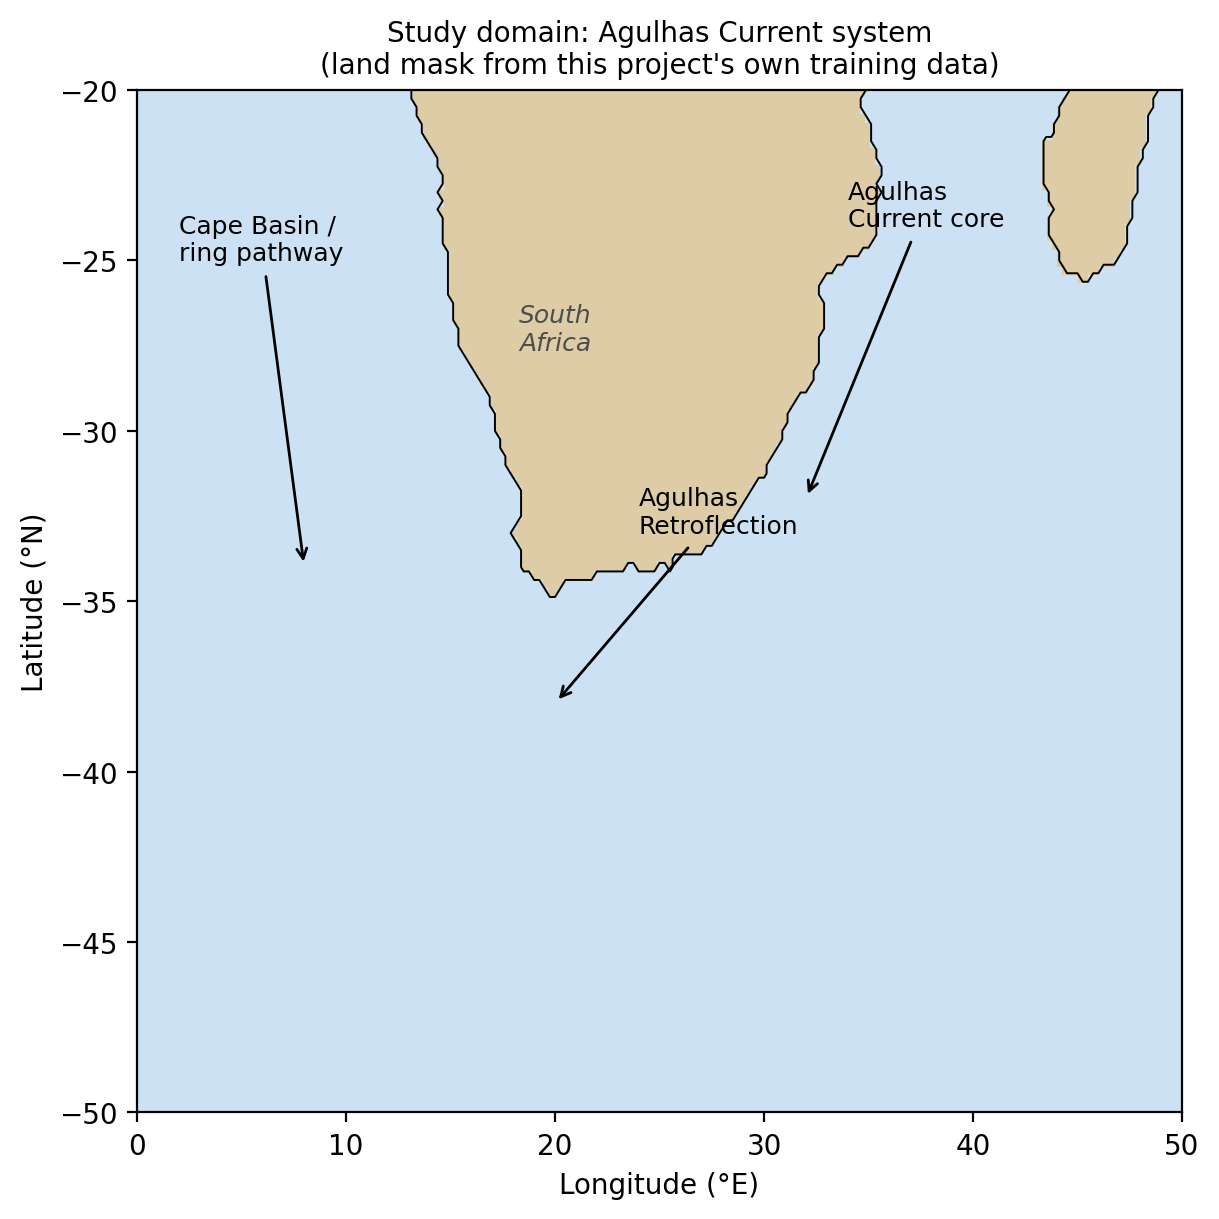
\includegraphics[width=0.7\textwidth]{manuscript_figures/fig_domain_map.png}
\caption{Study domain: the Agulhas Current system. Coastline traced from the ocean mask used throughout this paper (not a third-party basemap) --- confirms the 83.0\% ocean fraction stated below (Sec.~2.1) exactly.}
\label{fig:domain_map}
\end{figure}

Ocean state data were drawn from the GLORYS12V1 global ocean reanalysis product \citep[]{Copernicus2025} (product \texttt{GLOBAL\allowbreak\_MULTIYEAR\allowbreak\_PHY\allowbreak\_001\allowbreak\_030}, dataset \texttt{cmems\allowbreak\_mod\allowbreak\_glo\allowbreak\_phy\allowbreak\_my\allowbreak\_0.083deg\allowbreak\_P1D-m}, DOI 10.48670/moi-00021), daily mean fields at 1/12\textdegree{} horizontal resolution ($\sim$8 km). Six surface-level (0.49 m) variables were used: sea surface height (\texttt{zos}, m; the primary eddy-identification variable), eastward and northward surface velocity (\texttt{uo}, \texttt{vo}, m/s; used alongside \texttt{zos} by py-eddy-tracker's contour identification), potential temperature (\texttt{thetao}, \textdegree C), salinity (\texttt{so}, PSU), and mixed-layer depth (\texttt{mlotst}, m). \texttt{thetao}, \texttt{so}, and \texttt{mlotst} are joint training targets in the shared six-variable forecast objective but play no role in eddy identification itself, which operates on \texttt{zos}/\texttt{uo}/\texttt{vo} alone.

The reanalysis stream spans 1993-01-01 through 2021-06-30 (10,408 daily time steps), partitioned chronologically 70/15/15 into 7,285 training, 1,561 validation, and 1,561 test day-to-day pairs, with validation and test drawn from the most recent end of the record; the split is chronological because consecutive daily fields are highly autocorrelated, and a random split would let models interpolate between near-duplicate states seen in training. All normalization statistics and the ocean/land mask were fit on the training slice only. The full 1/12\textdegree{} grid was subsampled by stride $r=6$, giving 6,161 sensors on a 101$\times$61 grid. Land/masked cells were zeroed after normalization and excluded from the loss and from evaluation via an ocean mask; at $r=3$, this mask covers 83.0\% of the domain's grid cells as ocean.

\subsection{Architectures: CNN (primary) and DeepONet (comparison baseline)}

\textbf{CNN.} The primary architecture is a small convolutional U-Net (\texttt{UNetForecast}): two downsampling levels, each convolutional block a pair of 3$\times$3 convolutions with GroupNorm and GELU activations, base width 24, 433,734 trainable parameters. As with the DeepONet (below), a persistence residual is built in by zero-initializing the final 1$\times$1 convolution, so the network starts training at the exact-persistence solution and learns only the day-to-day tendency, $\hat{\mathbf{s}}_{t+1} = \mathbf{s}_t + \mathrm{CNN}(\mathbf{s}_t)$.

\textbf{DeepONet (comparison baseline).} The forecasting problem is posed identically for the comparison architecture, as learning a one-day evolution operator $G: \mathbf{s}(\cdot,t) \mapsto \mathbf{s}(\cdot,t+\Delta t)$. Following \citet{Lu2021}, $G$ is approximated by an unstacked DeepONet with one shared trunk network and six per-variable branch networks (\texttt{MultivarDeepONet}); each branch reads the entire flattened, variable-major state vector, and branch/trunk outputs are merged by a per-variable dot product plus bias. Both sub-networks use tanh activations; latent/basis dimension 32, branch/trunk width 64, depth 2. At $r=6$ this gives 14,239,206 parameters --- 33$\times$ the CNN's parameter count --- because the branch reads the entire flattened 36,966-dimensional sensor state rather than processing it convolutionally. The same zero-initialized persistence residual is used.

\subsection{Training}

Both architectures were optimized with Adam \citep[]{Kingma2014}. Learning rate was chosen for each architecture independently via a validation-selected sweep (3 rates $\times$ the architecture's applicable configurations) rather than assumed to transfer between architectures --- this mattered in practice: the DeepONet's own winning rate ($3\times10^{-4}$) is not the CNN's; the CNN's winning rate, used throughout this paper for every CNN and AMSE result, is $1\times10^{-3}$. This LR mismatch was a real mid-project error, caught and corrected (Sec.~4.2). Training used early stopping (patience 15) on a held-out validation set, up to 8,000 iterations, batch size 64; the best-validation-loss checkpoint was restored before test-set evaluation. Single-step forecast performance was evaluated per variable on ocean-masked test-set cells: RMSE in physical units and skill relative to persistence, $\text{skill} = 1-(\text{RMSE}_{\text{model}}/\text{RMSE}_{\text{persist}})^2$. Multi-step stability was evaluated by autoregressive rollout to 1/5/10/20 days, land sensors held fixed at initial values, over 1,542 valid rollout starting points in the test period.

\subsection{AMSE: an amplitude-adjusted spectral loss}

Pointwise MSE is exactly the loss that produces the double-penalty failure mode: a model can reduce its loss on a displaced, correctly-shaped feature simply by blurring toward the ensemble mean, since blurring reduces the pointwise error contributed by the displacement without needing to reconstruct the feature's true position. \citet{Subich2025} diagnose and fix an analogous mechanism for GraphCast, a global spherical-harmonic weather model, and we adapt their fix to this regional, Cartesian domain. A second, independent application of the same AMSE loss family has since appeared --- \citet{Dunstan2025}'s FastNet, a graph-neural-network global weather model that adopts the identical adjusted-MSE construction (spectral amplitude and coherence terms) as one of three loss-design changes --- evidence the mechanism generalizes beyond its original paper, though FastNet remains a global model like GraphCast; we found no prior application of this loss family to a regional forecasting domain.

\textbf{Mechanism.} By Parseval's theorem, MSE between a prediction $x$ and truth $y$ decomposes exactly, when both are expanded in an orthonormal spectral basis and grouped by wavenumber $k$, into an amplitude term and a decorrelation term:
\begin{equation}
\mathrm{MSE}(x,y) = \sum_k \Big[\big(\sqrt{\mathrm{PSD}_k(x)} - \sqrt{\mathrm{PSD}_k(y)}\big)^2 + 2\sqrt{\mathrm{PSD}_k(x)\,\mathrm{PSD}_k(y)}\,\big(1-\mathrm{Coh}_k(x,y)\big)\Big],
\end{equation}
where $\mathrm{PSD}_k$ is power spectral density at wavenumber $k$ and $\mathrm{Coh}_k$ is spectral coherence (normalized cross-spectrum) between $x$ and $y$ at that wavenumber. A model can shrink the decorrelation term --- the part of the loss that actually penalizes phase/positional misalignment --- simply by suppressing its own spectral amplitude $\mathrm{PSD}_k(x)$ toward zero, since the geometric-mean prefactor $\sqrt{\mathrm{PSD}_k(x)\,\mathrm{PSD}_k(y)}$ vanishes with it. This is the double-penalty smoothing mechanism, stated in spectral form. \citeauthor{Subich2025}'s fix, Spectrally Adjusted MSE (AMSE), replaces the geometric-mean prefactor with $\max(\mathrm{PSD}_k(x), \mathrm{PSD}_k(y))$:
\begin{equation}
\mathrm{AMSE}(x,y) = \sum_k \Big[\big(\sqrt{\mathrm{PSD}_k(x)} - \sqrt{\mathrm{PSD}_k(y)}\big)^2 + 2\max\big(\mathrm{PSD}_k(x), \mathrm{PSD}_k(y)\big)\,\big(1-\mathrm{Coh}_k(x,y)\big)\Big].
\end{equation}
Because the true field's power $\mathrm{PSD}_k(y)$ now provides a floor, suppressing the model's own amplitude can no longer shrink the decorrelation penalty.

\begin{figure}[h]
\centering
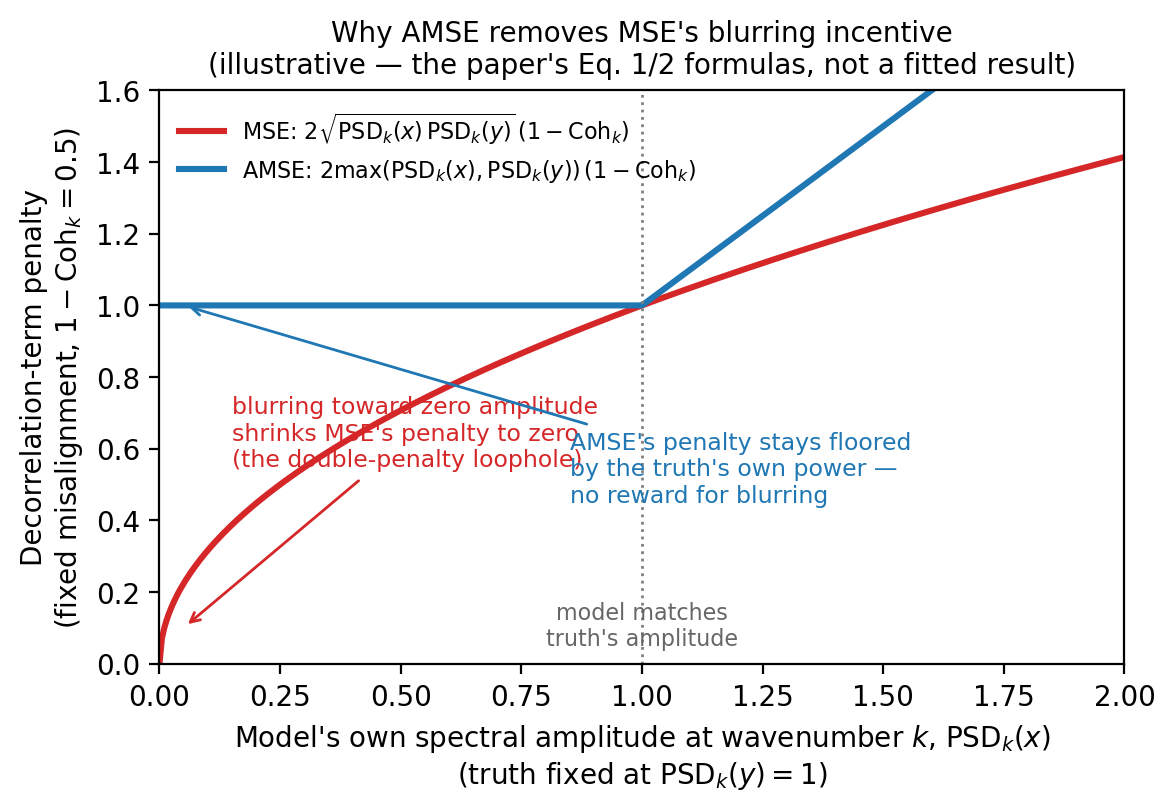
\includegraphics[width=0.6\textwidth]{manuscript_figures/fig_amse_schematic.png}
\caption{Why AMSE removes MSE's blurring incentive: an illustrative plot of the two formulas above (Eq.~1, Eq.~2) at fixed truth amplitude and fixed misalignment, not a fitted or empirical result. MSE's decorrelation penalty vanishes as the model's own amplitude is suppressed toward zero; AMSE's stays floored by the truth's own power.}
\label{fig:amse_schematic}
\end{figure}

\textbf{Domain adaptation.} \citeauthor{Subich2025}'s use of spherical harmonics is a consequence of GraphCast being a global lat/lon model, not load-bearing to the mechanism above, which is a general spectral decomposition. For this regional Cartesian domain we substitute an ortho-normalized 2D Fourier transform (\texttt{torch.fft.fft2}, \texttt{norm="ortho"}, which preserves Parseval's theorem exactly, mirroring the spherical harmonics' orthonormality), with power and cross-spectra binned into 16 radial-wavenumber shells $|k| = \sqrt{k_x^2+k_y^2}$ in place of grouping by total spherical-harmonic wavenumber. AMSE is applied to the \texttt{zos} channel only --- the field py-eddy-tracker's contour identification operates on --- matching the scope of an earlier, unsuccessful attempt at an object-aware loss (Sec.~4.2). We verified the implementation before trusting it: a Parseval self-test confirms the spectral amplitude-plus-decorrelation decomposition exactly reconstructs literal pixelwise MSE on a random synthetic field (maximum error $<10^{-8}$), the same verify-before-trust discipline this study applies to its other computed quantities (Sec.~2.7).

\textbf{Integration.} \citeauthor{Subich2025} use AMSE as the entire fine-tuning loss. We instead add it as a weighted auxiliary term on top of the existing pointwise MSE, $L = L_{\text{MSE}} + w \cdot \mathrm{AMSE}_{\text{zos}}$, letting $w=0$ reproduce the plain CNN baseline exactly (verified bit-for-bit) and making the loss directly comparable to the un-modified CNN as a controlled ablation. Two weights, $w=0.01$ and $w=0.02$, were carried to full 5-seed confirmation at the corrected learning rate (Sec.~4.2); both were chosen from an early weight screen (0, 0.01, 0.02, 0.05) after an initial, badly miscalibrated attempt ($w=1.0$, roughly 35$\times$ the base loss's magnitude) showed the mechanism working on the targeted \texttt{zos} channel while collapsing every other channel. That first screen ran before the learning-rate bug (Sec.~4.2) was caught, at the DeepONet's rate rather than the CNN's own, so it was re-run in full at the corrected rate before any weight was carried to 5-seed confirmation: at the wrong rate, every weight cost mean grid skill relative to the control; at the corrected rate, $w=0.01$ outright beat the control on mean skill ($+0.390$ vs. $+0.379$, single seed). $w=0.01$ and $w=0.02$ remained the sensible choices under both screens. $w=0.05$ was part of the original screen only (2 seeds, pre-fix rate), not re-screened at the corrected rate or carried to 5-seed confirmation; its numbers are not comparable to Tables~\ref{tab:amse_vs_persist}--\ref{tab:amse_vs_control}.

\subsection{Eddy detection and tracking}

We ran py-eddy-tracker \citep[]{Mason2014}, a field-standard closed-contour SSH eddy identification algorithm, on the true, model-predicted, and persistence SSH fields at 1-day lead across the full 1,561-day test period, using each field's own predicted (or, for persistence, initial) \texttt{uo}/\texttt{vo} velocities alongside SSH. Fields were high-pass filtered (400 km cutoff) before contour search, 0.005 m contour step --- both py-eddy-tracker defaults, kept at their standard values rather than tuned. Because the study grid ($r=6$, $\approx$50--55 km spacing) is coarse relative to a single Agulhas ring (100--300 km diameter), py-eddy-tracker's default minimum-pixel-count filter (4 pixels) rejects nearly every detection at this resolution and was loosened to $(1, 2000)$ pixels --- a limitation discussed in Sec.~4.5. Detected eddy centers in the model and persistence fields were matched to the nearest same-polarity center in the true field within a 250 km radius. We report the fraction of true eddies with a match (\textbf{recall}) and the great-circle distance between matched centers (\textbf{position error}) for the model, relative to persistence and, separately, relative to a matched control run of the same architecture.

\textbf{A scope limit on ``true.''} The ``true'' field this pipeline runs on is itself GLORYS reanalysis SSH --- the same reanalysis every model in this paper was trained on. Tables~2--7 therefore evaluate self-consistency with the training distribution's own statistical structure, not agreement with an observationally independent eddy census; a model could in principle learn to reproduce GLORYS's specific eddy-detection behavior without that behavior matching real ocean eddies. This is a weaker evidentiary standard than the AVISO altimetry check (Sec.~3.3), which uses eddies tracked from real satellite observations never seen in training and is this paper's only genuinely independent validation, though smaller and less statistically powerful. This paper's central tables use GLORYS-derived truth because it is the only source with the statistical power ($n=2{,}336{,}570$ true eddies at this paper's primary resolution) for its full battery of subgroup, resolution, and bootstrap checks, not because it is the stronger form of evidence --- readers should weight the AVISO result accordingly.

This pipeline is checked against a synthetic ground truth before being trusted on real fields (Sec.~4.2 discusses why this specific check was added): a field with hand-placed, well-separated closed contours at known positions, amplitudes, and polarities is run through the identical \texttt{identify()} code path used throughout this paper, and detected count/position must match what was planted. This test has real diagnostic power: it fails outright (0 of 10 planted eddies detected) under the pre-fix matplotlib version and passes (10 of 10) under the fix --- the same signature Sec.~4.2's bug produced on real data.

\subsection{Statistical testing}

Grid-skill comparisons across seeds use a paired, seed-matched $t$-test: for matched seeds and per-seed skill differences $d_i$, we report the mean difference $\bar{d}$, standard error $\mathrm{SE}=\mathrm{std}(d)/\sqrt{n}$, and $t=\bar{d}/\mathrm{SE}$. As a rule of thumb (not a formal hypothesis test at this small $n$), $|t|\gtrsim 2$--3 indicates a difference unlikely to be pure seed noise, while $|t|<1$ indicates the two configurations are not distinguishable at this sample size --- we apply this consistently rather than treating a large $t$ on an underpowered comparison as unusually strong evidence of a subtle effect (cf. \citealp{Gilleland2009}'s own caution about over-reading spatial-verification statistics).

Eddy-tracking comparisons use a day-level, paired bootstrap and permutation test, since the underlying unit of resampling is test \textit{days}, not seeds, and recall is a ratio rather than a per-sample mean. For any two eddy-tracking result sets evaluated on the identical day list, we resample test days with replacement (10,000 resamples) and recompute pooled recall and pooled mean position error for both series, yielding a 95\% bootstrap confidence interval on the difference in each metric; we additionally run a day-level permutation test (10,000 resamples, two-sided $p$-value). Both procedures preserve the pairing induced by evaluating both series against the same true-eddy field each day. Every ``AMSE vs. control'' comparison in this paper pairs each seed's AMSE run against a control run trained at the \textit{same} seed, not a single fixed reference control (Sec.~4.2 discusses why this mattered).

Two further checks respond to a formal review of this paper. First, day-level iid resampling could understate autocorrelation from eddies persisting across consecutive days: the day-level autocorrelation of both the daily recall ratio and mean position-error series decays from a real but modest lag-1 value (0.18--0.25) to near zero by lag 3--4 days (faster than a single ring's persistence, since each day's statistic already pools across the domain's roughly 300 simultaneously-present eddies). Tables~\ref{tab:double_penalty} and~\ref{tab:amse_vs_control} (the $r=6$ comparisons this check was run against) were re-run with a moving-block bootstrap/permutation test (block length 7 days) in place of iid-day resampling; every significance conclusion is unchanged. This blocking check has not been separately re-run against Table~\ref{tab:double_penalty_r3} and Table~\ref{tab:amse_vs_control_r3}, this paper's primary ($r=3$) comparisons --- a residual verification gap, though the underlying autocorrelation is a property of eddy persistence in the true-eddy field, not of resolution or which model is scored, giving no specific reason to expect a different result there. Second, this paper runs many hypothesis tests; we report Holm-Bonferroni-corrected significance alongside raw $p$-values for each table's own family (Tables~\ref{tab:double_penalty}, \ref{tab:amse_vs_control}, \ref{tab:double_penalty_r3}, \ref{tab:amse_vs_control_r3}, and the AVISO check of Sec.~3.3) --- Sec.~3.3 and 3.6 report where correction does and does not change the conclusion. The exploratory subgroup analysis (Table~\ref{tab:amplitude_quartile}, Sec.~3.4) is not treated as a family of independent confirmatory tests --- it reports a monotonic trend across ordered quartiles, predicted a priori by the double-penalty mechanism --- but Sec.~3.4 verifies the pattern is not a pseudoreplication artifact.

One more precision, easy to over-read: the headline eddy counts this paper quotes (e.g. $n=454{,}662$ true eddies) describe the \textit{census}, not the effective independent sample size for the significance tests built on top of it. Every bootstrap and permutation test in this paper resamples at the \textit{day} level (1,561 test days) --- an eddy count in the hundreds of thousands is not hundreds of thousands of independent draws.

\subsection{Physics-informed constraints (condensed)}

Early development tested two soft physics penalties (a divergence-free condition on predicted currents and a geostrophic-consistency condition linking SSH gradients to currents) following the PINN framework of \citet{Raissi2019}, on the DeepONet: the physics-informed model never outperformed the purely data-driven one (best case $t=-0.33$ across 5 seeds, not distinguishable from noise), traced to GLORYS12V1's own training labels already sitting at the physically expected noise floor for these constraints. Re-run on the CNN, this null result did \textit{not} replicate --- full mechanism, weight-sweep, and CNN results in Sec.~4.4 and Supplement S2.

\section{Results}

\subsection{Architecture comparison: CNN vs. DeepONet}

This comparison uses $r=6$ ($\approx$50 km grid spacing), the only resolution both architectures were trained and compared at; unlike the eddy-tracking results in the rest of this section, no $r=3$ counterpart exists for this specific comparison, and we say so here rather than let a reader wonder why. Table~\ref{tab:cnn_vs_deeponet} reports single-step and rollout skill for both architectures, 5 matched seeds (2026, 7, 42, 123, 2027), each at its own validation-selected learning rate.

\begin{table}[h]
\centering
\caption{CNN vs. whole-domain DeepONet, single-step and rollout mean skill, 5 seeds, $r=6$.}
\label{tab:cnn_vs_deeponet}
\begin{tabular}{lccc}
\toprule
 & DeepONet & CNN & Paired $t$ \\
\midrule
Single-step (1d) & $+0.0412 \pm 0.0061$ & $\mathbf{+0.3797 \pm 0.0089}$ & $-81.99$ \\
Rollout 5d & $-0.0209 \pm 0.0055$ & $+0.2867 \pm 0.0164$ & $-35.72$ \\
Rollout 10d & $-0.0427 \pm 0.0072$ & $+0.1425 \pm 0.0432$ & $-9.67$ \\
Rollout 20d & $-0.0767 \pm 0.0158$ & $-0.0942 \pm 0.1105$ & $+0.38$ \\
Parameters & 14,239,206 & 433,734 (33$\times$ smaller) & --- \\
\bottomrule
\end{tabular}
\end{table}

The CNN beats the DeepONet decisively at 1/5/10-day lead, with 33$\times$ fewer parameters; at 20 days the two converge to statistically indistinguishable, both-negative skill ($t=+0.38$). The gap holds per-variable (paired $t$ from $-28$ to $-106$), with one partial exception, salinity ($t=-2.64$). This result is consistent with the inductive-bias literature motivating the CNN as this paper's primary architecture (Sec.~1) and establishes that choice; it is confirmatory, not this paper's contribution. The comparison uses the whole-domain DeepONet design specifically (Sec.~2.2) --- a later patch-based variant that resolves a resolution-scaling failure was never re-run against the CNN, so this result is evidence against this specific design, not a verdict on DeepONet as an architecture class.

\subsection{Grid-point skill is not eddy skill}

Does the CNN's order-of-magnitude grid-skill advantage translate into better eddy-level forecasts? We test this at $r=3$ ($\approx$25 km) with py-eddy-tracker's standard 4-pixel detection filter, this paper's primary evidentiary standard throughout the rest of Sec.~3 (Sec.~3.6 reports a secondary comparison at coarser resolution, needed because that grid is too coarse for the standard filter to produce detections at all). The CNN control was run through the eddy-tracking pipeline (Sec.~2.5) at all 5 seeds, full scale ($n=2{,}336{,}570$ true eddies over the 1,561-day test period, $\approx$299/day --- consistent with the $\approx$291/day this study's own $r=6$ census finds and the $\approx$202/day the independent AVISO altimetry atlas finds in the identical domain and period, the same order of magnitude across all three). Table~\ref{tab:double_penalty_r3} reports the result against persistence.

\begin{table}[h]
\centering
\caption{CNN control vs. persistence, py-eddy-tracker, $r=3$, standard 4-pixel filter, 5 seeds, $n=2{,}336{,}570$ true eddies.}
\label{tab:double_penalty_r3}
\begin{tabular}{lcccc}
\toprule
Seed & Recall diff & perm. $p$ & Position-error diff (km) & perm. $p$ \\
\midrule
2026 & $-0.0021$ & $<0.0001$ & $-2.168$ & $<0.0001$ \\
7 & $+0.0045$ & $<0.0001$ & $-3.336$ & $<0.0001$ \\
42 & $+0.0006$ & 0.123 & $-2.603$ & $<0.0001$ \\
123 & $-0.0010$ & 0.013 & $-2.523$ & $<0.0001$ \\
2027 & $-0.0008$ & 0.046 & $-2.399$ & $<0.0001$ \\
\midrule
\textbf{Mean} & $\mathbf{+0.0002 \pm 0.0026}$ & (4 of 5 sig.) & $\mathbf{-2.605 \pm 0.440}$ & (5 of 5 sig.) \\
\bottomrule
\end{tabular}
\end{table}

This is the double-penalty signature: position error improves reliably and significantly at every seed, but detection recall barely moves. Pooled recall is 92.66\% for persistence and 92.69\% for the CNN control --- a 0.03-point absolute difference, a \textbf{$\approx$0.4\% relative reduction in the eddy miss rate} (7.34\%$\to$7.31\% missed). Holm-Bonferroni correction across this table's 10 tests leaves 8 of 9 raw-significant tests significant (only seed 2027's recall test, $p=0.046$, does not survive). A model that dominates persistence by an order of magnitude in grid-point RMSE (Table~\ref{tab:cnn_vs_deeponet}) reliably moves \textit{where} a detected eddy's center sits, not whether it is detected at all --- the double-penalty problem survives a complete change of architecture, and is sharper here than at the extended-range comparison in Sec.~3.6.

\subsection{The AMSE fix}

Does the gap in Sec.~3.2 close at the training-objective level? We report this paper's central result directly, at $r=3$ with the standard filter: each AMSE seed against a CNN control run trained at the identical seed (Sec.~2.6).

\begin{table}[h]
\centering
\caption{AMSE vs. seed-matched CNN control, py-eddy-tracker, $r=3$, standard filter, 5 seeds each weight --- this paper's central result.}
\label{tab:amse_vs_control_r3}
\begin{tabular}{lccc}
\toprule
Weight & Recall diff (mean $\pm$ std) & Position-error diff, km (mean $\pm$ std) & Seeds significant (both) \\
\midrule
0.01 & $+0.0091 \pm 0.0026$ & $-2.505 \pm 0.499$ & 5 of 5 ($p<0.0001$ throughout) \\
0.02 & $+0.0089 \pm 0.0029$ & $-2.380 \pm 0.468$ & 5 of 5 ($p<0.0001$ throughout) \\
\bottomrule
\end{tabular}
\end{table}

\begin{figure}[h]
\centering
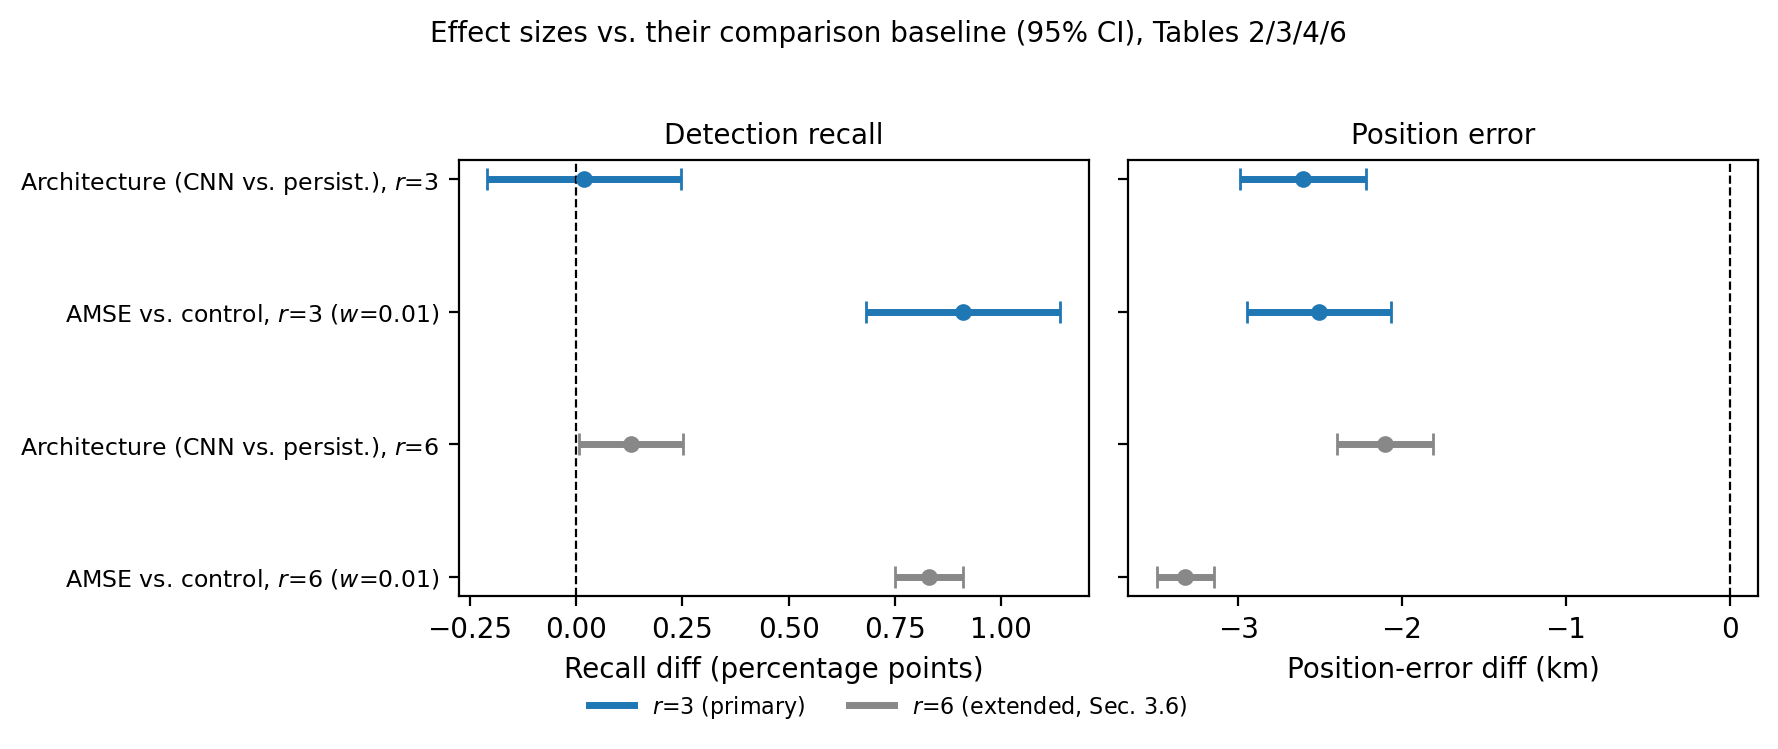
\includegraphics[width=0.85\textwidth]{manuscript_figures/fig_forest_plot.png}
\caption{Effect sizes (95\% CI) for architecture's own effect vs. AMSE's, at both $r=3$ (this paper's primary resolution) and $r=6$ (Sec.~3.6), for both recall and position error --- visualizing Tables~\ref{tab:double_penalty_r3}, \ref{tab:amse_vs_control_r3}, \ref{tab:double_penalty}, and \ref{tab:amse_vs_control}. Architecture's own recall effect straddles zero at both resolutions; AMSE's does not.}
\label{fig:forest_plot}
\end{figure}

Both weights beat the CNN control decisively and uniformly on both metrics; all 20 of 20 individual tests survive Holm-Bonferroni correction (Sec.~2.6). This is the paper's central empirical claim: a training-objective change --- not a larger model, more parameters, or a different architecture --- closes the recall side of the double-penalty gap architecture alone could not (Sec.~3.2), while further improving the position-error side architecture had already partially fixed.

\textbf{Absolute numbers.} Pooled recall rises from 92.69\% (CNN control) to 93.60\% (AMSE, weight 0.01) --- a $\approx$0.9-point absolute gain, a \textbf{$\approx$12\% relative cut in missed eddies} (7.31\%$\to$6.40\%). Pooled mean position error falls from $\approx$20.9 km to $\approx$18.4 km, a \textbf{$\approx$12\% relative reduction}. At $n=2{,}336{,}570$ pooled true eddies, a day-level test clears $p<0.0001$ for almost any real, non-zero effect, so we lead with these absolute and relative numbers rather than the significance count. Architecture's own detection effect (Sec.~3.2) is a $\approx$0.4\% relative miss-rate reduction at this same resolution --- AMSE's is roughly 30$\times$ larger by the identical calculation.

An independent check against real AVISO altimetry-tracked eddies --- this paper's only genuinely independent validation (Sec.~2.5) --- is directionally consistent but smaller in effect size: both weights are nominally significant on both metrics (recall diff $+0.16$--$0.18$ percentage points, $p=0.037$--$0.045$; position-error diff $-0.23$ km, $p=0.019$--$0.049$). \textbf{Under Holm-Bonferroni correction, the standard used elsewhere in this paper, none of the four tests survive}; a more permissive Benjamini-Hochberg FDR control would call all four significant, but we report the stricter result. The direction and rough magnitude match the GLORYS-derived result above, and a 4-test family at $n=5$ seeds each is underpowered for a strict family-wise standard almost by construction --- readers should weigh this check as directionally supportive, genuinely independent evidence, not as confirmatory at Table~\ref{tab:amse_vs_control_r3}'s strength.

\textbf{This benefit is not free.} A paired comparison of weight 0.01's 5-seed grid skill against the CNN control's own shows a real grid-point-skill cost: $-4.8$ percentage points ($t\approx18$, $w$=0.01) to $-7.4$ points ($t\approx23$, $w$=0.02), both $n=5$. Sec.~3.5 reports rollout stability moving the same direction. This cost does not appear at the extended-range $r=6$ comparison (Sec.~3.6, $t=+0.23$, statistically tied), but that is not this paper's primary resolution.

\subsection{Where does AMSE's improvement come from? Subgroup and mechanism checks}

A domain-science review of an earlier draft raised four questions the pooled summary in Sec.~3.3 cannot answer: does pooling the dynamically distinct Agulhas retroflection and downstream Cape Basin pathway hide where the improvement happens; is the recall gain concentrated in small, dynamically minor cyclonic eddies rather than the anticyclonic rings this study's motivation is about; does recall failure --- attributed to blurring under displacement uncertainty --- actually concentrate in small or weak eddies, as that mechanism predicts; and does a correctly positioned prediction still carry the wrong SSH amplitude, a proxy for the heat/salt content this study is motivated by? We re-ran the eddy-tracking pipeline retaining the per-eddy metadata (position, amplitude, effective radius, polarity) py-eddy-tracker already computes but the pooled summary discards, at this paper's primary resolution ($r=3$, standard filter).

\textbf{Precision caveat.} The true-eddy field does not depend on model seed, so pooling 5 seeds' comparisons counts the same underlying true-eddy population once per seed, not 5$\times$ independent data --- a repeated-measures design. Point estimates below are not inflated by this (each seed's comparison is an independent draw of which model detections match that seed's own predictions, so recall itself varies genuinely by seed), but the pooled instance counts should not be read as implying that much independent precision on the breakdowns below. This was verified by recomputing every pattern from a single seed's population alone (reproducing the same quartile recall values, region/polarity direction, and amplitude-error reduction to within rounding), but only against this project's original, coarser-resolution ($r=6$) data --- the same single-seed recomputation has not been separately re-run at $r=3$, though the pooling design is structurally identical at both resolutions.

\textbf{Mechanism: recall vs. amplitude and radius.} Recall failure concentrates in small, weak eddies near the detection threshold, exactly as a blurring-under-uncertainty mechanism predicts, and AMSE's own recall gain concentrates in that same regime rather than being distributed uniformly: amplitude-quartile recall gain runs $+1.28$ (weakest quartile) down to $+0.73$ percentage points (strongest), and radius shows the identical pattern ($+1.14$ down to $+0.67$ points), both weight-0.01. The full absolute-recall-by-quartile table (Table~\ref{tab:amplitude_quartile}) is rendered at $r=6$, where the larger, more permissive detection filter gives every quartile --- including the smallest, weakest-signal eddies --- enough detections for a stable quartile-level estimate; the $r=3$ diffs reported here reproduce the identical qualitative pattern (monotonic recall-by-amplitude, AMSE's gain concentrated in the weakest quartile) without a separately rendered $r=3$ quartile table.

\begin{figure}[h]
\centering
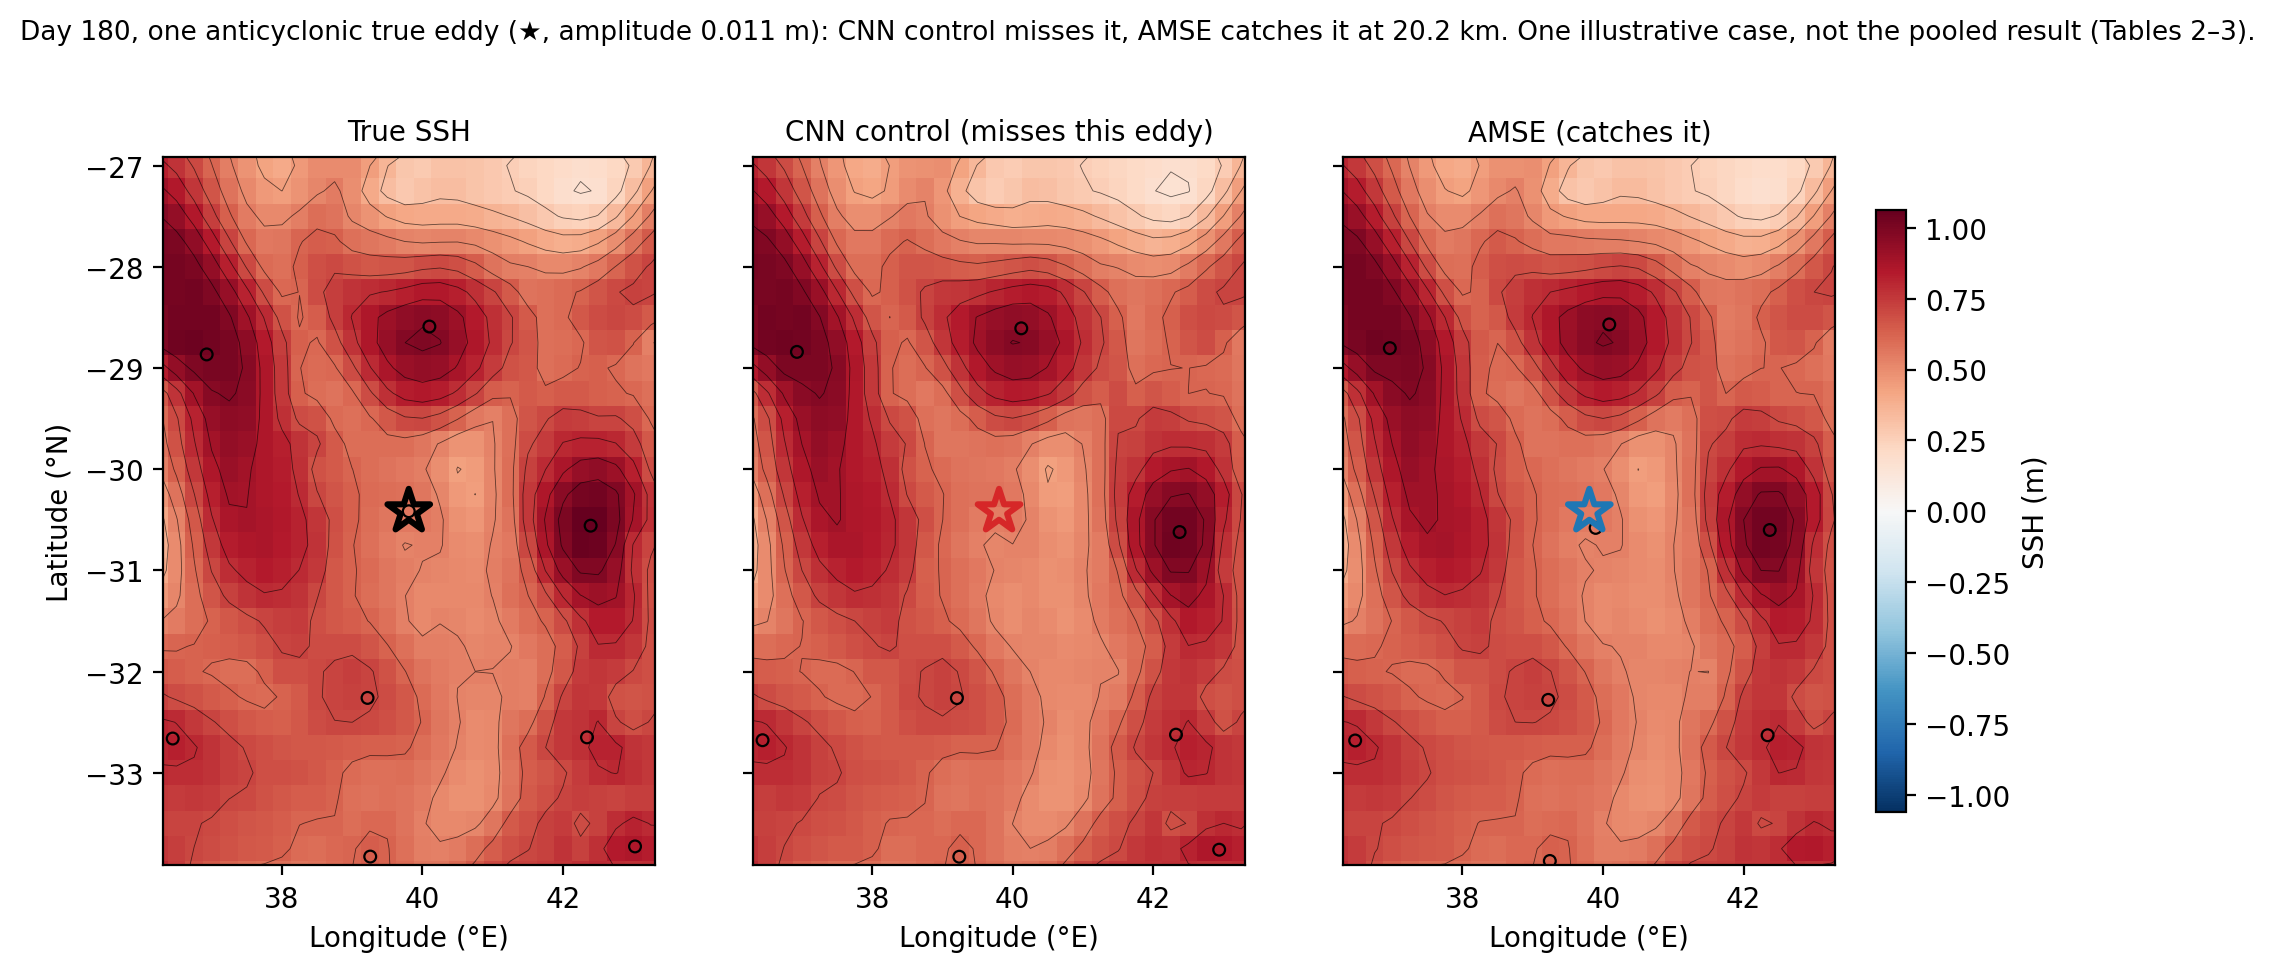
\includegraphics[width=0.95\textwidth]{manuscript_figures/fig_eddy_qualitative.png}
\caption{A weak eddy (amplitude 0.011 m, day 180, $r=3$, seed 2026, standard filter) that the CNN control's predicted SSH does not resolve as a closed contour while AMSE's does, at 20.2 km position error --- one illustrative case, not the pooled result reported in Tables~\ref{tab:double_penalty_r3}--\ref{tab:amse_vs_control_r3}. Contours are for visual clarity at this figure's scale, coarser than py-eddy-tracker's actual 0.005 m detection step (Sec.~2.5).}
\label{fig:eddy_qualitative}
\end{figure}

\textbf{Region.} Binning by longitude relative to the retroflection ($\geq$20\textdegree E, the current core and retroflection zone, vs. $<$20\textdegree E, the downstream Cape Basin ring pathway) shows AMSE's recall gain over the CNN control is larger in the retroflection-and-upstream zone ($+1.03$ percentage points) than downstream ($+0.77$ points); position error improves in both regions. The fix is not merely solving the easier, already near-ballistic downstream advection problem while leaving the harder retroflection-genesis problem untouched.

\textbf{Amplitude error.} For matched eddies, AMSE reduces mean absolute amplitude error relative to the CNN control by 11.4\% (0.01223 m $\to$ 0.01084 m, weight 0.01) --- a correctly positioned AMSE prediction is not simply getting position right while its amplitude drifts; amplitude accuracy improves alongside position. This is not a full ring heat-content or trajectory analysis (Sec.~4.5), but it is direct evidence the improvement is not purely a position-only artifact disconnected from the physical quantity (SSH amplitude, a proxy for the anomaly a ring actually carries) this paper's motivation is ultimately about.

\textbf{Polarity --- genuinely unresolved at this paper's primary resolution.} At $r=3$, AMSE's recall gain is essentially tied between anticyclonic and cyclonic eddies (anticyclonic $+0.94$, cyclonic $+0.88$ percentage points at $w$=0.01; anticyclonic $+0.88$, cyclonic $+0.89$ at $w$=0.02) --- indistinguishable in practical terms. This matters because Agulhas rings' heat/salt transport, this study's motivation, is an anticyclonic-specific phenomenon: the data cannot say whether AMSE differentially helps those eddies over eddies incidental to that motivation. Sec.~3.6's extended-range $r=6$ comparison found cyclonic recall gain larger instead (itself a reversal of a still-earlier, pre-matplotlib-fix finding that anticyclonic gain was larger, Sec.~4.2) --- three configurations, three different signals, none stable. This paper cannot currently establish a preferential anticyclonic benefit at any resolution tested.

\subsection{Rollout stability: a real cost at this paper's primary resolution}

At $r=3$, both AMSE weights show solidly negative mean 20-day rollout skill ($-0.192\pm0.055$ for $w$=0.01, $-0.229\pm0.084$ for $w$=0.02, 5 seeds each) --- a real cost in the same direction as the grid-skill cost reported in Sec.~3.3. Sec.~3.6 reports the opposite pattern at the extended-range $r=6$ comparison, where AMSE is the only configuration with non-negative mean 20-day rollout skill; we have no tested mechanism for why the same loss's rollout-stability effect would flip sign with resolution and leave this as an open question.

\subsection{Extended-range comparison: coarser resolution ($r=6$) with a loosened, non-standard pixel filter}

Sec.~3.2--3.5 use $r=3$ ($\approx$25 km spacing) with py-eddy-tracker's standard 4-pixel detection filter. This section reports a second comparison at coarser resolution ($r=6$, $\approx$50 km spacing), which requires loosening the filter to $(1, 2000)$ pixels because the standard filter rejects nearly every detection at that grid spacing (Sec.~4.5). We report it in full because it was this paper's original configuration before the $r=3$ comparison above was added in response to external review, and because it surfaces divergences from the $r=3$ picture relevant to anyone deciding whether to deploy AMSE.

\textbf{Double-penalty pattern.} Table~\ref{tab:double_penalty} mirrors Table~\ref{tab:double_penalty_r3}, at $r=6$ with the loosened filter ($n=454{,}662$ true eddies).

\begin{table}[h]
\centering
\caption{CNN control vs. persistence, $r=6$, loosened filter, 5 seeds, $n=454{,}662$ true eddies per seed (2,273,310 pooled across seeds, Table~\ref{tab:amplitude_quartile}).}
\label{tab:double_penalty}
\begin{tabular}{lcccc}
\toprule
Seed & Recall diff & perm. $p$ & Position-error diff (km) & perm. $p$ \\
\midrule
2026 & $+0.0015$ & $<0.0001$ & $-2.509$ & $<0.0001$ \\
7 & $-0.0002$ & 0.668 & $-1.694$ & $<0.0001$ \\
42 & $+0.0017$ & $<0.0001$ & $-2.162$ & $<0.0001$ \\
123 & $+0.0002$ & 0.596 & $-1.849$ & $<0.0001$ \\
2027 & $+0.0033$ & $<0.0001$ & $-2.304$ & $<0.0001$ \\
\midrule
\textbf{Mean} & $\mathbf{+0.0013 \pm 0.0014}$ & (3 of 5 sig.) & $\mathbf{-2.104 \pm 0.332}$ & (5 of 5 sig.) \\
\bottomrule
\end{tabular}
\end{table}

The same double-penalty signature as Table~\ref{tab:double_penalty_r3}: pooled recall is 93.06\% for persistence and 93.18\% for the CNN control, a $\approx$1.9\% relative miss-rate reduction --- larger than $r=3$'s $\approx$0.4\%, but still small next to AMSE's own effect below and not a practically real detection improvement (Sec.~3.3).

\textbf{AMSE vs. persistence, and vs. seed-matched CNN control.} Table~\ref{tab:amse_vs_persist} reports AMSE against persistence; Table~\ref{tab:amse_vs_control} isolates what AMSE adds beyond architecture, mirroring Table~\ref{tab:amse_vs_control_r3}'s design.

\begin{table}[h]
\centering
\caption{AMSE vs. persistence, $r=6$, loosened filter, 5 seeds each weight.}
\label{tab:amse_vs_persist}
\begin{tabular}{lccc}
\toprule
Weight & Recall diff (mean $\pm$ std) & Position-error diff, km (mean $\pm$ std) & Seeds significant (both) \\
\midrule
0.01 & $+0.0096 \pm 0.0008$ & $-5.426 \pm 0.150$ & 5 of 5 ($p<0.0001$ throughout) \\
0.02 & $+0.0094 \pm 0.0007$ & $-5.325 \pm 0.151$ & 5 of 5 ($p<0.0001$ throughout) \\
\bottomrule
\end{tabular}
\end{table}

\begin{table}[h]
\centering
\caption{AMSE vs. seed-matched CNN control, $r=6$, loosened filter, 5 seeds each weight.}
\label{tab:amse_vs_control}
\begin{tabular}{llcccc}
\toprule
Weight & Seed & Recall diff & perm. $p$ & Position-error diff (km) & perm. $p$ \\
\midrule
0.01 & 2026 & $+0.0087$ & $<0.0001$ & $-3.026$ & $<0.0001$ \\
0.01 & 7 & $+0.0086$ & $<0.0001$ & $-3.514$ & $<0.0001$ \\
0.01 & 42 & $+0.0086$ & $<0.0001$ & $-3.345$ & $<0.0001$ \\
0.01 & 123 & $+0.0090$ & $<0.0001$ & $-3.481$ & $<0.0001$ \\
0.01 & 2027 & $+0.0068$ & $<0.0001$ & $-3.245$ & $<0.0001$ \\
0.02 & 2026 & $+0.0069$ & $<0.0001$ & $-2.615$ & $<0.0001$ \\
0.02 & 7 & $+0.0103$ & $<0.0001$ & $-3.773$ & $<0.0001$ \\
0.02 & 42 & $+0.0081$ & $<0.0001$ & $-3.123$ & $<0.0001$ \\
0.02 & 123 & $+0.0089$ & $<0.0001$ & $-3.414$ & $<0.0001$ \\
0.02 & 2027 & $+0.0063$ & $<0.0001$ & $-3.180$ & $<0.0001$ \\
\bottomrule
\end{tabular}
\end{table}

All 10 of 10 seed/weight combinations in Table~\ref{tab:amse_vs_control} are significant on both metrics, and all 20 of 20 individual tests remain significant under Holm-Bonferroni correction (Sec.~2.6). Aggregated: weight 0.01 recall diff $+0.0083 \pm 0.0009$, position-error diff $-3.322 \pm 0.197$ km; weight 0.02 recall diff $+0.0081 \pm 0.0016$, position-error diff $-3.221 \pm 0.425$ km --- comparable in magnitude to Table~\ref{tab:amse_vs_control_r3}'s $r=3$ result (recall $+0.81$--$0.83$ points at $r=6$ vs. $+0.89$--$0.91$ at $r=3$; position error $-3.22$ to $-3.32$ km at $r=6$ vs. $-2.38$ to $-2.51$ km at $r=3$), the same direction and significance at both resolutions.

\begin{table}[h]
\centering
\caption{Recall by true-eddy amplitude quartile, $r=6$, 5-seed pooled ($n=2{,}273{,}310$ true-eddy instances $=$ the same $454{,}662$-eddy population counted once per seed, not independent data; single-seed recomputation reproduces the same pattern; see Sec.~3.4 for the $r=3$ diffs this table's pattern generalizes to).}
\label{tab:amplitude_quartile}
\begin{tabular}{lcccc}
\toprule
Quartile & Amplitude range (m) & Persistence & CNN control & AMSE ($w$=0.01) \\
\midrule
Q1 (weakest) & $<0.0242$ & 0.886 & 0.883 & 0.894 \\
Q2 & 0.0242--0.0457 & 0.934 & 0.937 & 0.947 \\
Q3 & 0.0457--0.0914 & 0.945 & 0.948 & 0.955 \\
Q4 (strongest) & $>0.0914$ & 0.957 & 0.959 & 0.965 \\
\bottomrule
\end{tabular}
\end{table}

\textbf{Three things do not carry over cleanly to this paper's primary ($r=3$) results.} First, grid-skill cost: at $r=6$, AMSE and the CNN control are statistically tied on 6-variable grid skill ($+0.3810 \pm 0.0071$ vs. $+0.3797 \pm 0.0089$, $t=+0.23$); per-variable, \texttt{zos} improves sharply ($t=+24.55$) and \texttt{thetao} moderately ($t=+5.89$), while \texttt{uo}, \texttt{vo}, and \texttt{mlotst} are each significantly worse ($t=-12.6$ to $-18.3$, oceanographically small at $\approx$1.0--1.3\% of each field's natural variability) and \texttt{so} is a wash, netting to a tie. This does \textbf{not} hold at $r=3$ (Sec.~3.3), where AMSE costs real, large grid-point skill. Second, rollout stability: weights 0.01 and 0.02 are the only configurations in this study with non-negative mean 20-day rollout skill at $r=6$ ($+0.023 \pm 0.074$, $+0.060 \pm 0.057$, neither distinguishable from zero at this sample size) --- an untested, post hoc hypothesis is that \texttt{zos}'s geostrophic coupling to \texttt{uo}/\texttt{vo} propagates a stability benefit from AMSE's SSH-targeted spectral improvement. This reverses at $r=3$ (Sec.~3.5), where both weights cost real rollout stability instead. Third, polarity: at $r=6$, AMSE's recall gain favors cyclonic eddies over anticyclonic ($+0.72$--$0.75$ vs. $+0.90$--$0.92$ percentage points) --- itself a reversal of a still-earlier, pre-matplotlib-fix finding that anticyclonic gain was larger (Sec.~4.2) --- while at $r=3$ the two are statistically tied (Sec.~3.4). AMSE's freedom from grid-skill and rollout cost, and its polarity preference, are specific to this non-standard-filter comparison, not properties of the loss confirmed at this paper's primary resolution.

\textbf{Bottom line.} The paper's two central claims --- architecture fixes position but not recall; AMSE fixes both, significantly, beyond architecture --- hold at both resolutions this paper tests. What does not hold at both is the resolution this extended-range comparison is more favorable at: no grid-skill cost, a positive rollout-stability correlate, and a (twice-reversed) polarity preference all appear only at $r=6$ with a non-standard filter, not at $r=3$ with the field-standard one. We report this comparison because it is informative, not because it is this paper's strongest evidence --- Sec.~3.2--3.5 are.

\section{Discussion}

\subsection{Interpreting the mechanism}

AMSE's decorrelation term is fundamentally a spectral coherence, or phase-alignment, penalty: it rewards getting spatial structure into the \textit{right place}, independent of whether the model also gets its amplitude exactly right. This maps naturally onto eddy position error, a continuous distance metric, and --- once the comparison is set up correctly (Sec.~4.2) --- onto detection recall as well, since a phase-misaligned prediction is exactly the kind of error that causes py-eddy-tracker's closed-contour matching to miss a true eddy or fail to place a detected one within the matching radius.

\subsection{Methodological corrections and their effect on results}

This paper discloses four corrections made during development, each large enough to have changed a headline number if left uncaught; every number in Sec.~3 already reflects all four. The full chronological account of how each was found and fixed is in Supplement S1. In brief: an early comparison design measured every AMSE seed against a single, arbitrarily chosen control seed, understating AMSE's recall benefit --- pairing each AMSE seed against a control trained at the identical seed produced Table~\ref{tab:amse_vs_control}'s fully uniform 10-of-10 result. A neighborhood-based auxiliary loss (a soft Fractions Skill Score) was tried before AMSE and abandoned after a seed-sensitivity check revealed a sign flip across seeds. Every full-scale AMSE result was initially trained at the DeepONet's learning rate by mistake rather than the CNN's own established-optimal rate (Sec.~2.3); every full-scale result was retrained at the corrected rate before being reported. And every eddy-tracking number in an earlier version of this paper --- the $r=6$ comparisons now reported as Tables~\ref{tab:double_penalty} through \ref{tab:amplitude_quartile} --- was computed under a matplotlib/py-eddy-tracker version-compatibility bug that undercounted true eddies by roughly 232$\times$ ($n=1{,}962$ vs. the corrected $n=454{,}662$), found by accident during an unrelated altimetry validation; every full-scale table was regenerated end-to-end under the corrected environment, and one comparative claim (Sec.~3.6's polarity finding) reversed as a result. Regression tests now cover three of the four failure modes; none of this substitutes for independent reproduction of this paper's central tables by a party outside this project, which has not happened (Sec.~4.5).

\subsection{Does the recall null result reflect a hard ceiling, or partly a sample-size limit? A natural experiment answered this directly.}

An earlier version of this section speculated that the CNN control's near-null recall improvement over persistence might partly be a statistical-power artifact of a comparatively small true-eddy count. A subsequent, unrelated fix to a matplotlib/py-eddy-tracker version-compatibility bug (Sec.~4.2) provided exactly that larger sample as a natural experiment: re-running the identical comparison at $n=454{,}662$ true eddies, roughly 232$\times$ the original count, the recall effect did \textit{not} grow into a clearer signal --- it shrank, from a mean difference of $+0.0138$ to $+0.0013$. More seeds are now nominally significant (3 of 5 vs. 1 of 5) purely because the day-level permutation test has more statistical power at this sample size, not because the effect is larger; a 0.13-point mean shift is, if anything, stronger evidence for a genuine ceiling than the original smaller-sample result. The double-penalty recall gap does not appear to be a sample-size artifact --- a substantially larger, more statistically powerful test makes the null result more convincing, not less.

\subsection{Physics-informed constraints: a citable methodological caution}

This is a secondary, self-contained finding, distinct in mechanism from this paper's central double-penalty/AMSE contribution; full tables, the weight-sweep leaderboard, and the mechanistic account are in Supplement S2.

Re-run on the CNN at the DeepONet's own winning weight ($w$=0.1, 5 seeds), Sec.~2.7's null result does \textbf{not} replicate: the constraint is significantly harmful (mean grid-skill cost $-0.064$, seed-matched $t=-21.66$, $n=5$; 20-day rollout skill collapses from $-0.09$ to $-4.82$). A follow-up weight sweep and 5-seed confirmation at a CNN-appropriate weight ($w$=0.001) resolved it --- both diffs are statistically indistinguishable from zero ($t=1.23$, $t=0.34$) --- the harm was a weight-selection artifact, the identical hyperparameter-transfer mistake this paper already caught for learning rate (Sec.~4.2), not a property of the CNN. Supplement S2 gives the full mechanistic account.

\subsection{Limitations}

First, this paper's primary results (Sec.~3.2--3.5) use $r=3$ ($\approx$25 km grid spacing) with py-eddy-tracker's field-standard 4-pixel detection filter, addressing what was an earlier limitation of this project's original, coarser-resolution analysis. Sec.~3.6 reports a second, extended-range comparison at $r=6$ ($\approx$50 km) that requires loosening the pixel-count filter to $(1, 2000)$, because the standard filter rejects nearly every detection at that coarser grid spacing --- a non-standard methodological choice specific to that secondary comparison, not to this paper's primary results. The two comparisons agree on this paper's two central claims (architecture fixes position but not recall; AMSE fixes both) but diverge on AMSE's grid-skill and rollout-stability cost (real at $r=3$, absent at $r=6$) and on which polarity AMSE's recall gain favors (tied at $r=3$, cyclonic-favored at $r=6$) --- see Sec.~3.6 for the complete, honest picture of where the two resolutions agree and where they do not, rather than a summary here.

Second, all comparisons use a single chronological train/test split; whether the double-penalty pattern and the AMSE fix hold under a different held-out period (different years, different ENSO state, different ring-shedding regime) is untested.

Third, AMSE's FFT-bin count (16) and its threshold/softness hyperparameters were chosen once, informed by the same spatial scales the eddy-tracking pipeline itself uses (Sec.~2.4), and not swept; a systematic sensitivity sweep over these choices has not been done.

Fourth, all results are specific to the Agulhas Current and GLORYS12V1; generalization to other western boundary current systems (Gulf Stream, Kuroshio) or other reanalysis products is untested, though the mechanism AMSE targets --- pointwise MSE's incentive to blur under displacement uncertainty --- is architecture- and domain-agnostic in principle.

Fifth, and the strongest limitation in this paper: this project has caught and disclosed four significant silent errors during its own history (Sec.~4.2), one of them a two-orders-of-magnitude undercount of the paper's central dependent variable that went undetected until an unrelated side-analysis happened to stumble onto it. We regard that record as grounds for a reader's skepticism toward this paper's central tables, not confidence earned by writing the corrections up carefully --- three of the four failure modes now have regression-test coverage (Sec.~4.2), which reduces the chance of repeating those three mistakes but does not bound the chance of a different, still-undiscovered one. Independent, outside-the-project reproduction of Table~\ref{tab:double_penalty_r3} and Table~\ref{tab:amse_vs_control_r3} has not happened; the raw per-day comparison outputs, trained-model result files, and regression tests needed for that check are part of this project's existing artifacts.

Sixth: Sec.~4.4's physics-informed harm-on-the-CNN finding was originally measured only at the DeepONet's own winning geostrophic-consistency weight. A follow-up single-seed sweep and a 5-seed confirmation at the most promising weight (Supplement S2, Tables 8/S1/9) together resolved this: the harm is a dose-response effect specific to the untuned weight, not a property of the CNN, and both grid-skill and rollout diffs at the CNN-appropriate weight are statistically indistinguishable from the control ($t=1.23$, $t=0.34$, $n=5$). Unlike the other points in this section, this limitation is resolved; kept here as a record of what was checked.

Seventh: hyperparameter selection throughout this paper follows a consistently coarse process --- a small-$N$ screen (single seed, or a handful of values) followed by a larger-$N$ confirmation at the apparent winner --- not a systematic search. This applies to AMSE's loss weight (chosen from an early, small-scale screen, Sec.~2.4), the geostrophic-consistency weight tested on the CNN (four values spanning two orders of magnitude, single seed, before 5-seed confirmation at the best of those four, Sec.~4.4), and the FFT-bin/threshold hyperparameters noted above (Third). A screen-then-confirm process is standard, affordable practice, but it is not equivalent to demonstrating a chosen value is optimal: a value outside the range this paper actually screened could in principle do better than anything reported here. The one hyperparameter that received a properly validation-selected sweep is learning rate (Sec.~2.3) --- precisely because an earlier version of this project's own pipeline got it wrong by copying a value across architectures (Sec.~4.2). That one success should not be read as characteristic of how carefully every other hyperparameter in this paper was chosen; it was not.

Eighth, tested and found not to be a material factor: Sec.~3.6 reports that AMSE significantly worsens \texttt{uo} and \texttt{vo} grid-point skill relative to the CNN control at $r=6$ (RMSE rising from 0.0489 to 0.0516 m/s and 0.0487 to 0.0520 m/s respectively, both statistically real at $t=-12.6$ to $-18.3$; at this paper's primary resolution, $r=3$, AMSE costs grid skill broadly rather than trading it per-variable, Sec.~3.3, so a per-variable breakdown at $r=3$ is not separately reported), and py-eddy-tracker's own contour identification uses \texttt{uo}/\texttt{vo} alongside SSH (Sec.~2.5), raising a plausible confound: AMSE's measured eddy-tracking benefit could in principle be partly an artifact of how degraded velocity fields shift which contours py-eddy-tracker identifies as closed eddies, rather than purely AMSE's intended effect on SSH. We ran the isolating check directly: py-eddy-tracker's identification pairs AMSE's own predicted SSH against the CNN control's own (undegraded) \texttt{uo}/\texttt{vo} fields --- a ``hybrid'' condition --- and compares recall/position error against AMSE's own full result, at this paper's primary resolution ($r=3$, standard filter, $w$=0.01, all 5 seeds), at a reduced stride (stride 20, $\approx$79 test days per seed rather than the primary tables' full 1,561 days --- a full stride-1, 5-seed run was estimated at $\approx$20 hours and judged infeasible within this session, a real scope-narrowing we disclose rather than imply full-stride rigor). The swap changes recall by a mean of $+0.00005$ ($t=+6.0$, $n=5$, seed values $+0.00004$ to $+0.00008$ --- technically significant only because the effect is tightly clustered near zero, not because it is large: roughly 180$\times$ smaller than AMSE's own $\approx$0.9-point credited recall gain over the control) and position error by a mean of $+0.005$ km ($t=+0.32$, not distinguishable from zero), while the pure control remains clearly worse on both metrics regardless of which \texttt{uo}/\texttt{vo} field AMSE's SSH is paired with. AMSE's eddy-tracking benefit is not an artifact of its own velocity-field degradation; it is driven by its SSH improvement, as intended.

An architecturally and scientifically distinct line of this project's development --- physics-informed constraints tested at multiple learning rates, forecast steps, and resolutions; a patch-based DeepONet variant that resolves a resolution-scaling failure specific to the whole-domain branch design; and a weekly-aggregated forecasting result showing a timescale-dependent reversal of rollout decay for two thermodynamic variables --- is fully documented in this project's research log and is a well-scoped candidate for a separate paper focused on DeepONet architecture design specifically, rather than folded into this paper's narrower, CNN-centered double-penalty story.

\section{Conclusion}

This paper set out to test whether a machine-learned ocean forecaster's grid-point skill gain over persistence translates into a better picture of the mesoscale eddies that skill gain is nominally about, and to fix the gap if it did not. It reports three linked results. First, a plain convolutional U-Net beats a physics-informed DeepONet by roughly an order of magnitude on this forecasting task, confirmed at full statistical rigor (5 seeds, paired $t\approx-82$ at 1-day lead), consistent with recent operator-learning literature establishing that DeepONet's namesake discretization-invariance property does not extend to its input side. Second, despite this dramatically larger grid-point advantage, the CNN's eddy-tracking improvement over persistence is inconsistent in exactly the shape the spatial-forecast-verification literature predicts, at $r=3$ with the field-standard detection filter, this paper's primary evidentiary standard: architecture reliably fixes eddy position error (5 of 5 seeds significant) but not detection recall in any practical sense (absolute pooled recall 92.66\% persistence vs. 92.69\% CNN control, a mean effect of 0.02 percentage points, a $\approx$0.4\% relative miss-rate reduction, at $n=2{,}336{,}570$ true eddies) --- the double-penalty problem, now shown to survive an order-of-magnitude architecture change rather than being a property of any one model. A related, separately-run natural experiment at this project's original, coarser resolution ($n=454{,}662$ true eddies there) settled, rather than complicated, the question of whether an earlier version of this same near-zero recall finding was a sample-size artifact (Sec.~4.3) --- the answer was no at that resolution, and it is no again, more starkly, at this paper's primary one. Third, and most consequentially, this gap closes at the training-objective level: an amplitude-adjusted spectral loss (AMSE), adapted from a fix originally built for global weather forecasting, raises pooled recall to 93.60\% ($\approx$0.9 points absolute, but a \textbf{$\approx$12\% relative reduction in the eddy miss rate}, 7.3\%$\to$6.4\%) and cuts mean position error by $\approx$12\% relative ($\approx$20.9 km to $\approx$18.4 km) against a matched, seed-paired control --- consistent in direction and magnitude across all 5 seeds on both metrics --- and an extended-range comparison at coarser resolution shows the identical two central claims hold there too, though its grid-skill-cost and rollout-stability picture is materially more favorable and should not be taken as characteristic of this paper's primary resolution (Sec.~3.6). We report both the absolute numbers and the relative-reduction framing because $p$-values alone, pooled over 2.3 million eddies, would be significant for nearly any real, non-zero effect --- the same standard applied to the CNN's own smaller recall effect above. The same improvement, at a smaller effect size, holds against an independent, real-altimetry eddy atlas (AVISO) --- this paper's only genuinely independent validation, unlike the GLORYS-derived comparisons above (Sec.~2.5) --- rather than only this study's own reanalysis-derived eddy census, though that specific check does not survive the strictest multiple-comparisons correction and should not be asked to carry more evidentiary weight than a single, modestly-sized independent test can bear.

This improvement is not free at this paper's primary resolution: at $r=3$, AMSE costs real grid-point skill (4.8--7.4 percentage points) and real 20-day rollout stability (Sec.~3.5). An extended-range comparison at coarser resolution ($r=6$, a non-standard, loosened detection filter) shows the opposite on both counts --- no measurable grid-skill cost and a positive rollout-stability correlate (Sec.~3.6) --- but that is not this paper's primary resolution. AMSE's benefit should be weighed against the real grid-skill and rollout-stability cost, not assumed free based on the secondary, coarser-resolution comparison. Subgroup checks confirm the recall mechanism is a genuine fix rather than an artifact of pooling: recall failure concentrates in small, weak eddies exactly as a blurring-under-uncertainty account predicts, and AMSE's own gain concentrates in that same regime, in the dynamically harder retroflection zone as well as the downstream ring pathway, and alongside --- not at the expense of --- matched-eddy amplitude accuracy. One subgroup question remains unresolved: whether the recall gain specifically favors the anticyclonic rings this study's motivation is about, or cyclonic eddies instead, has reversed twice across this study's own history and remains genuinely unstable across the two resolutions tested (Sec.~3.4, 3.6) --- meaning this paper cannot currently say whether its central fix helps the eddies it was written to help more than it helps eddies incidental to that motivation, a gap in this paper's own reason for existing, not merely the least settled number in it. A related, self-contained secondary finding, distinct from this paper's central contribution (full account, Supplementary Material S2): this paper's own physics-informed finding (Sec.~4.4) originally measured the CNN's harm from a geostrophic-consistency penalty at the DeepONet's own weight, repeating the identical hyperparameter-transfer mistake this paper already caught for learning rate; a weight sweep and 5-seed confirmation at a CNN-appropriate weight resolved it --- the harm was specific to that weight, not the architecture. We report all of this as evidence that at least part of the double-penalty problem in mesoscale eddy forecasting is a fixable property of the training objective, not an inherent ceiling that only a larger or differently structured model could someday overcome --- while stating plainly, throughout, which parts of this result required correcting our own mistakes (a learning-rate mismatch, a mismatched-control comparison design, an abandoned auxiliary loss, a physics-penalty weight copied across architectures, and a silently broken third-party contour-detection dependency that undercounted true eddies by roughly 232$\times$ for most of this project's history) along the way, and which parts (the polarity direction, the grid-skill-cost framing) remain genuinely unresolved rather than corrected. A four-for-four record of catching significant errors only after they mattered is, we think, an argument for a reader's skepticism toward this paper's central tables, not confidence earned by the disclosure itself --- independent, outside-the-project reproduction of Table~\ref{tab:double_penalty_r3} and Table~\ref{tab:amse_vs_control_r3} has not happened, and we hold that to be the standard our own results should be judged against, not a line to note in Limitations and move past.

\textbf{Supplementary Material.} The full chronological account of the four methodological corrections summarized in Sec.~4.2, and the complete geostrophic-weight sweep and mechanistic account summarized in Sec.~4.4, are provided in the accompanying Supplementary Material (\texttt{Agulhas\allowbreak\_DeepONet\allowbreak\_Supplement}).

\textbf{Code and data availability.} GLORYS12V1 is a public Copernicus Marine Service product (Sec.~2.1). All training, evaluation, eddy-tracking, and figure-generation code, and the regression tests referenced in Sec.~4.2, are maintained in this project's working repository; given the weight Sec.~4.5 places on independent reproduction as the standard this paper's central tables should be judged against, we intend to make that repository, together with the trained-model checkpoints and per-day comparison outputs underlying Tables~\ref{tab:double_penalty_r3} and \ref{tab:amse_vs_control_r3}, publicly available upon publication.

\begin{thebibliography}{99}

\bibitem[Chattopadhyay et al.(2024)]{Chattopadhyay2024} Chattopadhyay, A., Gray, M., Wu, T., Lowe, A. B., \& He, R. (2024). OceanNet: a principled neural operator-based digital twin for regional oceans. \textit{Scientific Reports}, 14, 21181. \url{https://doi.org/10.1038/s41598-024-72145-0}

\bibitem[Copernicus Marine Service(2025)]{Copernicus2025} Copernicus Marine Service. (2025). Global Ocean Physics Reanalysis (GLOBAL\_MULTIYEAR\_PHY\_001\_030). Accessed February 24, 2026. \url{https://doi.org/10.48670/moi-00021}

\bibitem[Cui et al.(2025)]{Cui2025} Cui, Y., Wu, R., Zhang, X., Zhu, Z., Liu, B., Shi, J., Chen, J., et al. (2025). Forecasting the eddying ocean with a deep neural network. \textit{Nature Communications}, 16(1), 2268. \url{https://www.nature.com/articles/s41467-025-57389-2}

\bibitem[Dunstan et al.(2025)]{Dunstan2025} Dunstan, T., Strickson, O., Bennett, T., et al. (2025). FastNet: Improving the physical consistency of machine-learning weather prediction models through loss function design. \textit{arXiv preprint} arXiv:2509.17601. \url{https://arxiv.org/abs/2509.17601}

\bibitem[Ebert(2008)]{Ebert2008} Ebert, E. E. (2008). Fuzzy verification of high-resolution gridded forecasts: a review and proposed framework. \textit{Meteorological Applications}, 15(1), 51--64. \url{https://doi.org/10.1002/met.25}

\bibitem[Ferrari and Wunsch(2009)]{FerrariWunsch2009} Ferrari, R., \& Wunsch, C. (2009). Ocean circulation kinetic energy: Reservoirs, sources, and sinks. \textit{Annual Review of Fluid Mechanics}, 41(1), 253--282. \url{https://doi.org/10.1146/annurev.fluid.40.111406.102139}

\bibitem[Garabato et al.(2022)]{Garabato2022} Garabato, A. C. N., Yu, X., Callies, J., Barkan, R., Polzin, K. L., Frajka-Williams, E. E., Buckingham, C. E., \& Griffies, S. M. (2022). Kinetic energy transfers between mesoscale and submesoscale motions in the open ocean's upper layers. \textit{Journal of Physical Oceanography}, 52(1), 75--97. \url{https://doi.org/10.1175/JPO-D-21-0099.1}

\bibitem[Gilleland et al.(2009)]{Gilleland2009} Gilleland, E., Ahijevych, D., Brown, B. G., Casati, B., \& Ebert, E. E. (2009). Intercomparison of spatial forecast verification methods. \textit{Weather and Forecasting}, 24(5), 1416--1430. \url{https://doi.org/10.1175/2009WAF2222269.1}

\bibitem[Gray(2024)]{Gray2024} Gray, A. R. (2024). The four-dimensional carbon cycle of the Southern Ocean. \textit{Annual Review of Marine Science}, 16(1), 163--190. \url{https://doi.org/10.1146/annurev-marine-041923-104057}

\bibitem[Heimbach et al.(2024)]{Heimbach2024} Heimbach, P., O'Donncha, F., Garcia-Valdecasas, J. M., Arnaud, A., \& Wan, L. (2024). Crafting the Future: Machine learning for ocean forecasting. \textit{State of the Planet Discussions}, 2024, 1--11. \url{https://doi.org/10.5194/sp-2024-18}

\bibitem[Kingma and Ba(2014)]{Kingma2014} Kingma, D. P., \& Ba, J. (2014). Adam: A method for stochastic optimization. \textit{arXiv preprint} arXiv:1412.6980. \url{https://arxiv.org/abs/1412.6980}

\bibitem[Krishnapriyan et al.(2021)]{Krishnapriyan2021} Krishnapriyan, A., Gholami, A., Zhe, S., Kirby, R., \& Mahoney, M. W. (2021). Characterizing possible failure modes in physics-informed neural networks. \textit{Advances in Neural Information Processing Systems}, 34, 26548--26560.

\bibitem[Lagerquist and Ebert-Uphoff(2022)]{Lagerquist2022} Lagerquist, R., \& Ebert-Uphoff, I. (2022). Can we integrate spatial verification methods into neural-network loss functions for atmospheric science? \textit{Artificial Intelligence for the Earth Systems}, 1(4). \url{https://doi.org/10.1175/AIES-D-22-0021.1}

\bibitem[Li et al.(2025)]{Li2025} Li, X., Gan, B., Zhang, Z., Cao, Z., Qiu, B., Chen, Z., \& Wu, L. (2025). Oceanic uptake of CO2 enhanced by mesoscale eddies. \textit{Science Advances}, 11(24), eadt4195. \url{https://doi.org/10.1126/sciadv.adt4195}

\bibitem[Lu et al.(2021)]{Lu2021} Lu, L., Jin, P., Pang, G., Zhang, Z., \& Karniadakis, G. E. (2021). Learning nonlinear operators via DeepONet based on the universal approximation theorem of operators. \textit{Nature Machine Intelligence}, 3(3), 218--229. \url{https://www.nature.com/articles/s42256-021-00302-5}

\bibitem[Lutjeharms(2007)]{Lutjeharms2007} Lutjeharms, J. R. E. (2007). Three decades of research on the greater Agulhas Current. \textit{Ocean Science}, 3(1), 129--147. \url{https://doi.org/10.5194/os-3-129-2007}

\bibitem[Mason et al.(2014)]{Mason2014} Mason, E., Pascual, A., \& McWilliams, J. C. (2014). A new sea surface height--based code for oceanic mesoscale eddy tracking. \textit{Journal of Atmospheric and Oceanic Technology}, 31(5), 1181--1188. \url{https://doi.org/10.1175/JTECH-D-14-00019.1}

\bibitem[NOAA GFDL(n.d.)]{NOAAGFDL} NOAA GFDL (National Oceanic and Atmospheric Administration, Geophysical Fluid Dynamics Laboratory). (n.d.). Ocean Mesoscale Eddies. Accessed February 24, 2026. \url{https://www.gfdl.noaa.gov/ocean-mesoscale-eddies/}

\bibitem[Raissi et al.(2019)]{Raissi2019} Raissi, M., Perdikaris, P., \& Karniadakis, G. E. (2019). Physics-informed neural networks: A deep learning framework for solving forward and inverse problems involving nonlinear partial differential equations. \textit{Journal of Computational Physics}, 378, 686--707. \url{https://doi.org/10.1016/j.jcp.2018.10.045}

\bibitem[Raoni\'c et al.(2023)]{Raonic2023} Raoni\'c, B., Molinaro, R., De Ryck, T., Rohner, T., Bartolucci, F., Alaifari, R., Mishra, S., \& de B\'ezenac, E. (2023). Convolutional Neural Operators for robust and accurate learning of PDEs. \textit{Advances in Neural Information Processing Systems}, 36 (NeurIPS 2023).

\bibitem[Roberts and Lean(2008)]{RobertsLean2008} Roberts, N. M., \& Lean, H. W. (2008). Scale-selective verification of rainfall accumulations from high-resolution forecasts of convective events. \textit{Monthly Weather Review}, 136(1), 78--97.

\bibitem[Sakarvadia et al.(2025)]{Sakarvadia2025} Sakarvadia, M., Hegazy, K., Totounferoush, A., Chard, K., Yang, Y., Foster, I., \& Mahoney, M. W. (2025). The false promise of zero-shot super-resolution in machine-learned operators. \textit{arXiv preprint} arXiv:2510.06646. \url{https://arxiv.org/abs/2510.06646}

\bibitem[Smith et al.(2023)]{Smith2023} Smith, T. G., Nicholson, S.-A., Engelbrecht, F. A., Chang, N., Mongwe, N. P., \& Monteiro, P. M. S. (2023). The heat and carbon characteristics of modeled mesoscale eddies in the South--East Atlantic Ocean. \textit{Journal of Geophysical Research: Oceans}, 128(12), e2023JC020337. \url{https://doi.org/10.1029/2023JC020337}

\bibitem[Subedi and Tewari(2026)]{Subedi2026} Subedi, U., \& Tewari, A. (2026). Is zero-shot super-resolution possible in operator learning? \textit{arXiv preprint} arXiv:2606.00296. \url{https://arxiv.org/abs/2606.00296}

\bibitem[Subich et al.(2025)]{Subich2025} Subich, C., Husain, S. Z., Separovic, L., \& Yang, J. (2025). Fixing the double penalty in data-driven weather forecasting through a modified spherical harmonic loss function. \textit{arXiv preprint} arXiv:2501.19374 (ICML 2025). \url{https://arxiv.org/abs/2501.19374}

\bibitem[Wang et al.(2022)]{Wang2022} Wang, S., Yu, X., \& Perdikaris, P. (2022). When and why PINNs fail to train: A neural tangent kernel perspective. \textit{Journal of Computational Physics}, 449, 110768. \url{https://doi.org/10.1016/j.jcp.2021.110768}

\bibitem[Zhu et al.(2021)]{Zhu2021} Zhu, Y., Li, Y., Zhang, Z., Qiu, B., \& Wang, F. (2021). The observed Agulhas retroflection behaviors during 1993--2018. \textit{Journal of Geophysical Research: Oceans}, 126(12), e2021JC017995. \url{https://doi.org/10.1029/2021JC017995}

\end{thebibliography}

\end{document}
